\chapter[Ferramenta de Gestao]{Ferramenta de Gestao}

Gestão de Tempo do Projeto é uma das principais áreas em Gerenciamento de Projetos, visto que é nessa etapa que são definidos os prazos e suas respectivas responsabilidades. Também é nessa fase que é apresentado o cronograma do projeto.

Embora seja possível criar um cronograma utilizando as tabelas do PowerPoint ou as planilhas do Excel, é muito mais prático utilizar softwares específicos para essa função, visto que eles permitem um acompanhamento não só dos prazos mas também de seus responsáveis e ligação entre os processos.

\section{Ferramenta}

Um dos softwares mais conhecidos para essa função é o Project, da Microsoft. O software, em suas últimas versões, permite não apenas a criação do cronograma e das tabelas de recursos, mas também a EAP, cronogramas macros, gestão de portfólio, etc. Esse software é pago e acaba sendo muito caro. A licença do MS Project 2010, a última versão, sai por cerca de R\$ 1.800,00. O que pode ser bastante desanimador para profissionais comuns e empresas menores, ou que não tenham uma maturidade de projetos avançada.

\subsection{Gantter}

Uma alternativa são alguns softwares genéricos, sendo alguns gratuitos. O Gantter é um app gratuito disponível na loja da Google.

O Gantter é uma poderosa ferramenta para Gerenciamento de Projetos baseada na internet, e por isso não requer instalação de nenhum software. Além disso, é completamente integrado com o Google Docs.

O Gantter permite criar e gerenciar projetos, criando recursos, calendários, tarefas críticas, planejamento de duração, trabalho e custo. Sua interface é bastante intuitiva, além de ser disponível em diversas línguas, inclusive o Português.

Com o Gantter é possível criar também Gráficos de Gantt criados originalmente por \cite{HLGANTT} são utilizados para gerenciamento de projetos pois permitem visualizar atividades e suas dependências em relação ao tempo.

O Gantter é um projeto pessoal do programador ucraniano \cite{VMazepa}, que desenvolveu a ferramenta para uso próprio depois de procurar e não encontrar nenhuma alternativa barata ou sem custos para o MS Project.

Sendo assim Gantter foi escolhido para ser utilizado como ferramenta de gestão do projeto de GPEQ: Pastelaria Bom Sabor.

\section{Cronograma}

\begin{figure}[H]
    \centering
  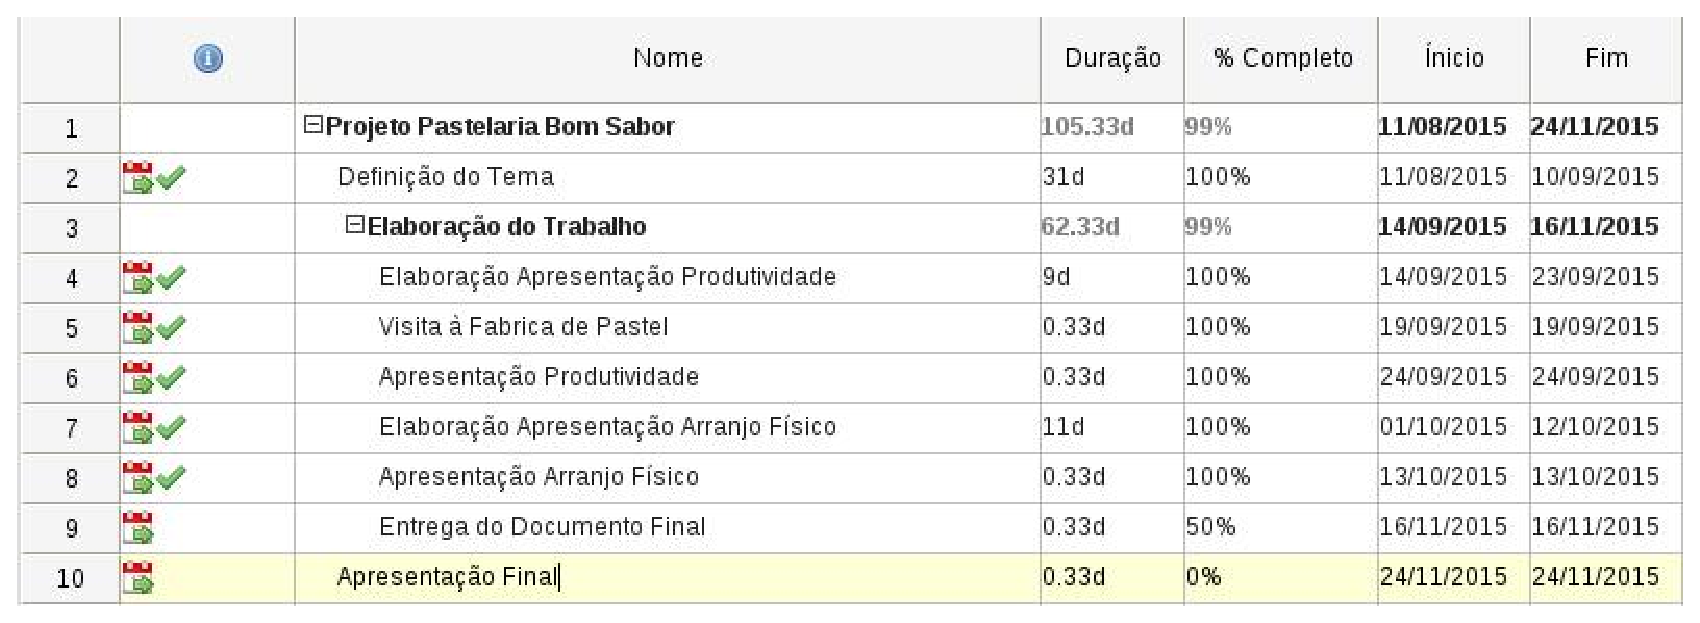
\includegraphics[keepaspectratio=true,scale=0.5]{figuras/cronograma.eps}
    \caption{Cronograma.}
    \label{fig:cronograma}
\end{figure}

\subsection{Gráfico de Gantt}

\begin{figure}[H]
    \centering
  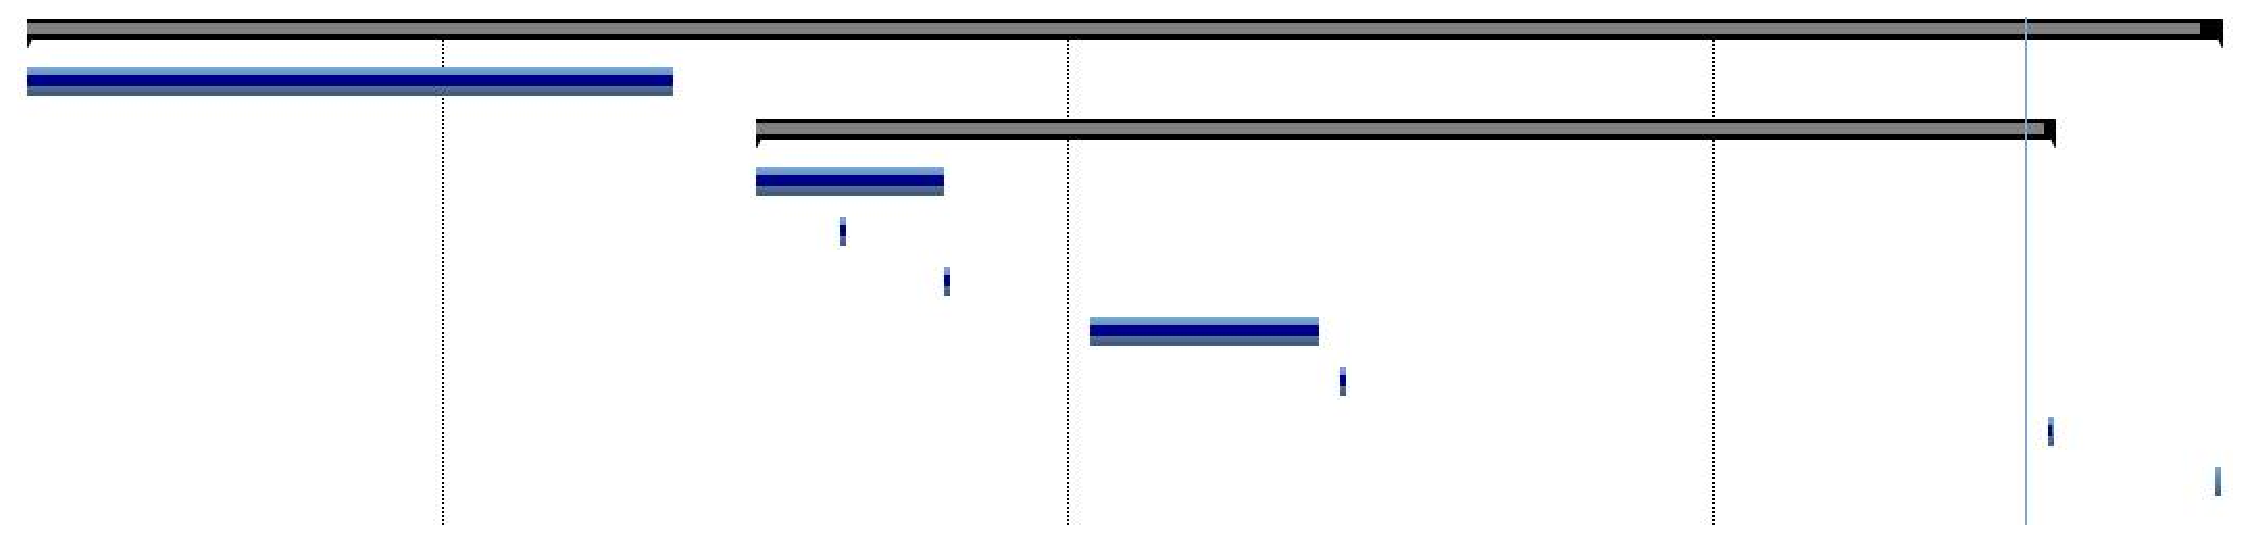
\includegraphics[keepaspectratio=true,scale=0.5]{figuras/grafico_gantt.eps}
    \caption{Gráfico de Gantt.}
    \label{fig:grafico_gantt}
\end{figure}